\chapter{Der Morse-Komplex}
In diesem Kapitel wird der Morse Komplex definiert und gezeigt, dass der 
Morse-Komplex ein Kettenkomplex ist.

\section{Die stabile- und instabile Mannigfaltigkeit und die Smale-Bedingung}

\begin{definition}[Stabile- und instabile Mannigfaltigkeit]
    \label{def: stabile und instabile mannigfaltigkeit}
    Es sei $f \colon M \to \R$ eine Morse-Funktion, $p$ ein kritischer Punkt von $f$ und $X$ ein
    Pseudo-Gradientenfeld von $f$. Die stabile Mannigfaltigkeit von $f$ ist die Menge
    \[ \stab (p) = \left\{ q \in M : \lim_{t \to + \infty} \phi_t(q) = p \right\} \]
    und die instabile Mannigfltigkeit ist
    \[ \unst (p) = \left\{ q \in M : \lim_{t \to - \infty} \phi_t(q) = p \right\} . \]
\end{definition}

Bevor wir die stabile- und instabile Mannigfaltigkeit eines kritischen Punktes weiter untersuchen, 
fixieren wir ein Paar Notationen zu Morse Umgebungen.

\begin{definition}[Notationen zu Morse Umgebungen]
    \label{def: notation morse umgebung}
    Zuerst untersuchen wir eine quadratische Form, die die Form hat wie Funktionen in Morse
    Umgebungen, also
    \[ Q \colon \R^n \to \R ; Q(x_1, \dots, x_n) = - x_1 - \dots - x_k + x_{k + 1} + \dots + x_n \]
    für ein $1 \leq k \leq n$.
    Mit $x_- := (x_1, \dots x_k) \colon \R^n \to \R^k$ und $x_+ := (x_{k + 1} \dots x_n)$ gilt dann
    \[ Q = - \| x_- \|^2 + \| x_+ \|^2 . \]
    Der Gradient von $Q$ ist mit dem Standardskalarprodukt auf $\R^n$
    \[ \grad Q (x_-, x_+) = 2(x_-, x_+) . \]
    Seien nun $\eps, \eta > 0$. Dann setzen wir
    \[ U(\eps, \eta) := \left\{ x \in \R^n : - \eps \leq Q(x) \leq \eps 
    \text{ und } \| x_- \|^2 \| x_+ \|^2 \leq \eta(\eps + \eta) \right\} := U \]
    Wir definieren außerdem
    \begin{align*}
        \del_{\pm} U := & \left\{ x \in U: Q(x) = \pm \eps \text{ und } \|x_{\mp} \|^2 \leq \eta \right\} 
            \text{ und} \\
        \del_0 U := & \left\{ x \in \del U: \| x_- \|^2 \| x_+ \|^2 = \eta(\eps + \eta) \right\} .
    \end{align*}
    Dann gilt 
    \[ \del U = \del_+ \cup \del_- \cup \del_0 . \]
    Wir setzen nun $V_- = \langle e_1, \dots, e_k \rangle$ und 
    $V_+ = \langle e_1, \dots, e_n \rangle \subseteq \R^n$. $V_+$ ist der größte Vektorraum, 
    auf dem $Q$ positiv definit ist und $V_-$ der größte Vektorraum, auf dem $Q$ negativ definit ist. 
    Es gilt 
    \[ \del U \cap V_{\pm} \subseteq \del_{\pm} U . \]

    Ist nun $f \colon M \to \R$ eine Morse Funktion, $p$ ein kritischer Punkt von $f$ und $(V, \psi)$
    eine Morse Umgebung von $p$, dann gilt $f \circ \psi^{-1} = Q + f(p)$. Sind $\eps$ und $\eta$
    klein genug, dann ist $U \subset \psi(V)$. Wir nennen $\Omega (p) = \psi^{-1}(U)$,
    $\del_{\pm} \Omega (p) = \psi^{-1}(\del_{\pm}U)$ und $\del_0 \Omega (p) = \psi^{-1} (\del_0 U)$.
    Dann ist 
    \[ \psi(\stab (p) \cap \Omega (p)) = V^+ \cap U \] 
    und 
    \[ \psi(\unst (p) \cap \Omega (p)) = V^- \cap U . \]
    Wir können uns also mit dieser Notation die stabile- und instabile Mannigfaltigkeit (wenigstens 
    in einer Umgebung von $p$) sehr gut vorstellen.

    \begin{figure}[H]
        \centering
        \begin{minipage}{.4\textwidth}
          \centering
          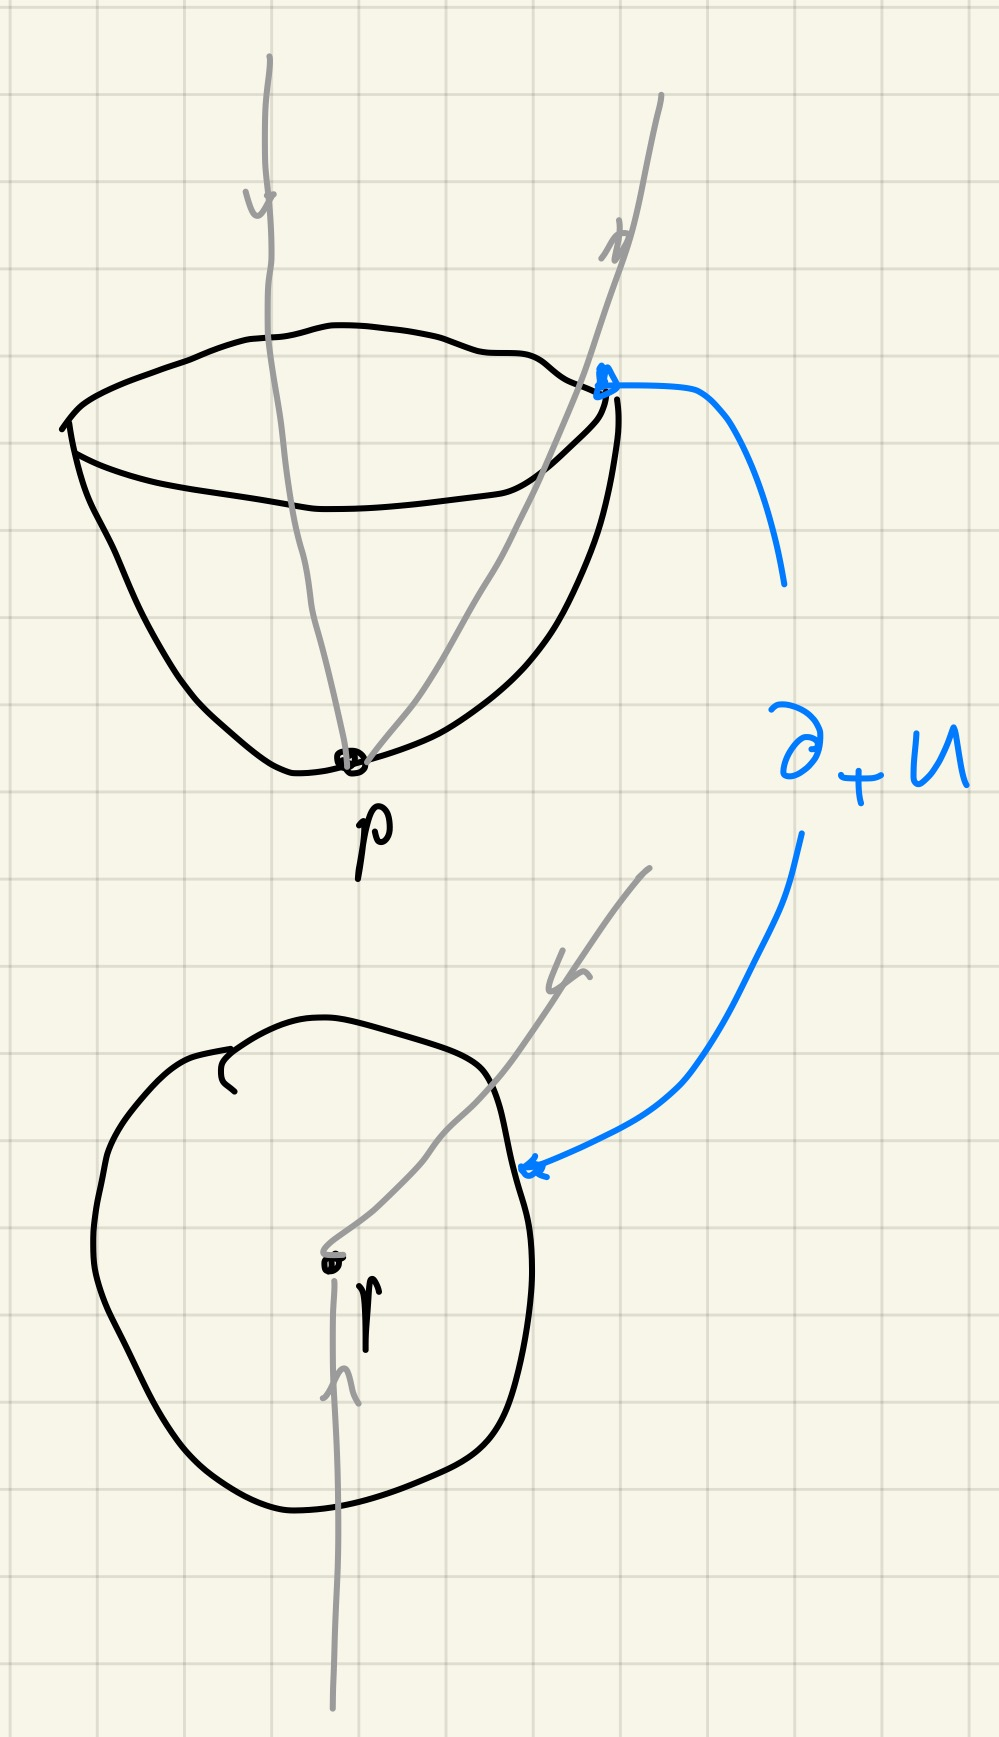
\includegraphics[width=.4\linewidth]{../resources/def-notation-morse-umgebung-1.JPG}
          \captionof{figure}{Index $0$}
          \label{fig: morse umgebung ind 0}
        \end{minipage}%
        \begin{minipage}{.4\textwidth}
          \centering
          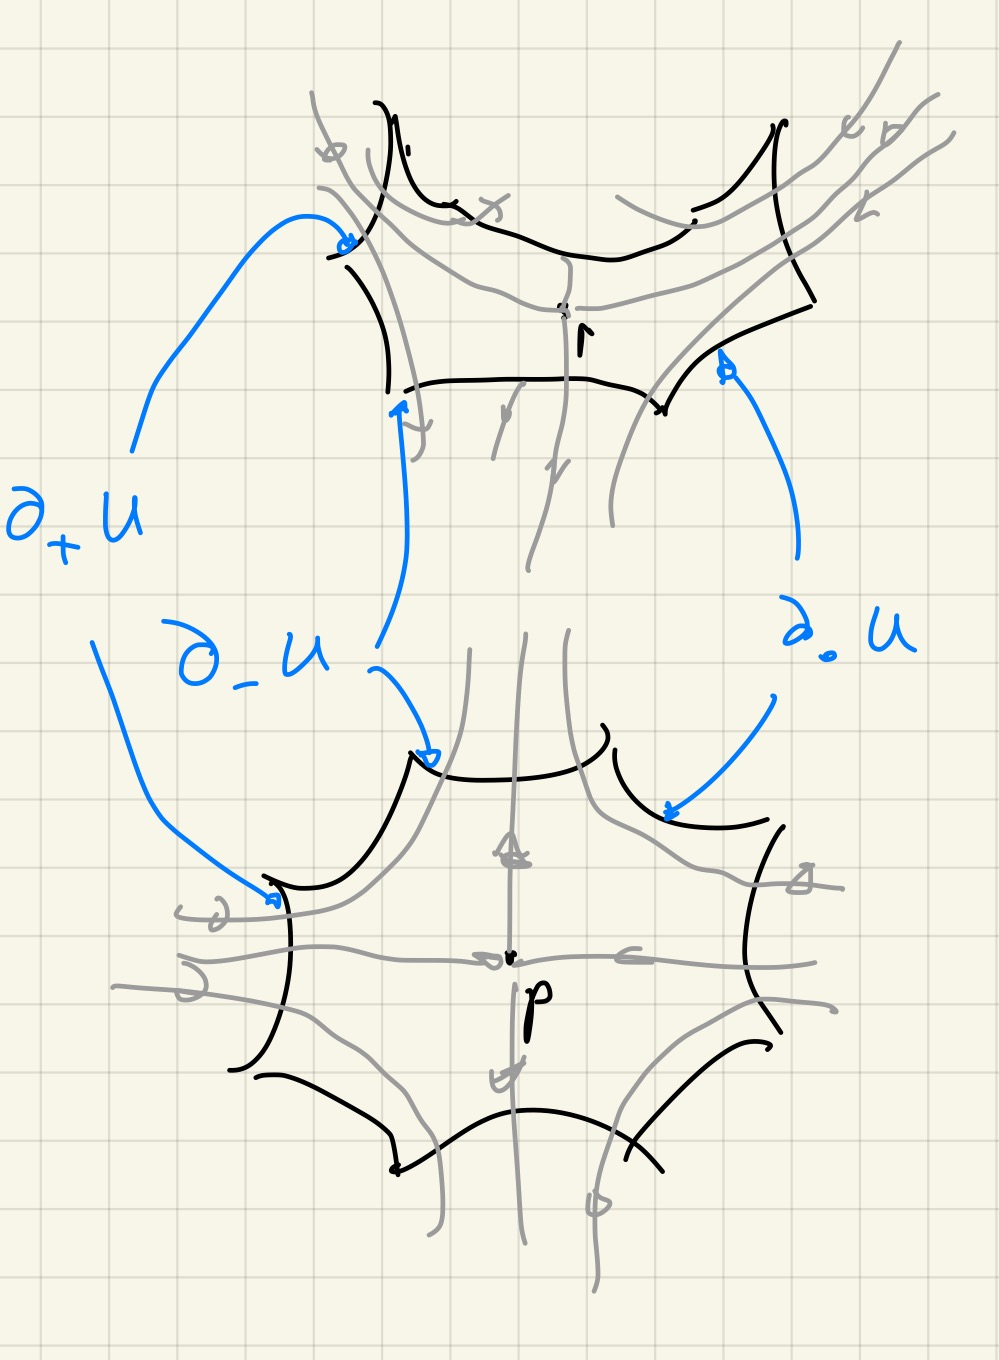
\includegraphics[width=.4\linewidth]{../resources/def-notation-morse-umgebung-2.JPG}
          \captionof{figure}{Index $k$, $0 < k < n$}
          \label{fig: morse umgebung ind k}
        \end{minipage}
    \end{figure}
\end{definition}

Wir sind nun bereit eine grundlegende aber wichtige Aussage zu beweisen.

\begin{prop}
    Ist $f \colon M \to \R$ eine Morse Funktion und $p$ ein kritischer Punkt von $f$, dann sind
    $\stab (p)$ und $\unst (p)$ Mannigfaltigkeiten mit 
    \[ \dim \unst (p) = n - \dim \stab (p) = \Index (p) \]
\end{prop}

\begin{proof}
    Es sei $(\psi, V)$ eine Morse Karte um $p$ in einer Form wie in ~\ref{def: notation morse umgebung},
    also sodass $\eps, \eta > 0$ exitstieren, sodass $\psi(V) = U(\eps, \eta) := U$. Es sei außerdem
    $\phi$ der Fluss eines Pseudo-Gradientenfeldes von $f$. Dann ist 
    \[ \Phi \colon \psi^{-1}(\del_+ U \cap V_+) \times \R \to M ; \psi(q, t) = \phi_t(q) \]
    eine Einbettung und es gilt 
    \[ \stab (p) = \Ima \Phi \cup \psi^{-1}(U \cap V_+) . \]
    Tatsächlich ist 
    \[ \stab (p) - \Ima \Phi = \{ p \} . \]
    Außerdem ist $\del_+ U \cap V_+ = \{ x \in \R^n: \| x_+ \|^2 = \eps \} \isom S^{n - k - 1}$, 
    denn für alle $x \in V_+$ gilt sowieso schon $x_- = 0$. Also ist $ \stab(p)$ diffeomorph zum Raum 
    $S^{n - k - 1} \times (-\infty, \infty]/\sim$, in dem alle Punkte in $\infty$ zusammengeklebt 
    werden. Dieser Quotient ist wiederum diffeomorph zur offenen Kreisscheibe mit Dimension $n - k$.
    Genauso zeigt man, dass $W^u (p)$ diffeomorph zur offenen Kreisscheibe mit Dimension $k$ ist.
\end{proof}

\begin{prop}
    \label{prop: trajektorien enden in kritischen punkten}
    Es sei $f \colon M \to \R$ eine Morse-Funktion und $X$ ein Pseudo-Gradientenfeld von $f$. 
    Sei außerdem $M$ kompakt. Ist dann $\phi$ der Fluss von $X$, dann existieren für jeden Punkt 
    $p \in M$ kritische Punkte $q$ und $r$ von $f$, sodass
    \[ \lim_{t \to + \infty} \phi_t(p) = q \;\;\; 
    \text{ und } \;\;\; \lim_{t \to -\infty} \phi_t(p) = r \]
\end{prop}

\begin{proof}
    Wir zeigen die erste Aussage. Seien für kritische Punkte $q$ $(U_q, \psi_q)$ die Karten, 
    auf denen der Pseudo Gradient mit dem negativen Gradienten auf $\R^n$ übereinstimmt. 
    Es ist $\lim_{t \to + \infty} \phi_t(p) = q$, genau dann wenn
    der Fluss $\phi_{\bullet}(p)$ den Punkt $p$ irgendwann in die Umgebung 
    $\del_+\psi_q(U_q) \cap \stab(q)$ transportiert. Angenommen $\phi_{\bullet}(p)$ transportiert
    $p$ nie zu einem kritischen Punkt. Jedes mal wenn $\phi_{\bullet}(p)$ also ins Innere einer
    Morse-Umgebung $U_q$ gerät, muss diese Umgebung auch wieder verlassen werden. Da 
    $f \circ \phi_{bullet}(p)$ monoton ist, kann nachdem $\phi_{bullet}(p)$ die Morse-Umgebung $U_q$
    verlassen hat, nie wieder zu dieser zurückgekehrt werden.
    Sei also 
    \[ U = \bigcup_{q \in \Crit(f)} U_q \]
    und $t_0$ der Zeitpunkt an dem $\phi_{\bullet} (p)$ die Umgebung $U$ das letzte mal verlässt.
    Da $M - U$ keine kritischen Punkte von $f$ enthält existiert ein $\eps_0 > 0$, sodass für alle 
    $x \in M - U$ gilt 
    \[ \opd f (x) ((X(x))) \leq - \eps_ . \]
    Wir rechnen also: Für jedes $t \geq t_0$ gilt
    \begin{align*}
        f(\varphi_t(p) - f(\varphi_{t_0}(p))) = & 
            \int_{t_0}^t \derive[f \circ \phi_{\bullet}(p)]{s} (s) \opd s \\
        = & \int_{t_0}^t \opd f (\phi_s(p)) (X(\phi_s(p))) \opd s \\
        \leq & - \eps_0 (t - t_0) . 
    \end{align*}
    Also für $t \to + \infty$ gilt $f(\phi_t(p)) \to - \infty$. Das kann aber nicht sein, denn da 
    $M$ kompakt ist muss auch $\Ima f$ kompakt sein. Also kann $\phi_{\bullet}(p)$ nicht alle 
    $U_q$ verlassen. aber dann ist 
    \[ \lim_{t \to + \infty} \phi_t(p) = q \]
    für einen kritischen Punkt $q$.
    Genauso zeigt man, dass $\lim_{t \to - \infty} \phi_t(p) = r$ für einen kritischen Punkt $r$.
\end{proof}

\begin{definition}[Smale-Bedingung]
    \label{def: smale-bedingung}
    Es sei $M$ eine Mannigfaltigkeit und $U$ und $V$ Untermannigfaltigkeiten von $M$. Wir sagen 
    $U$ und $V$ sind \textit{transversal} und schreiben $U \pitchfork V$, falls für alle Punkte 
    $p \in U \cap V$ gilt 
    \[ T_pU + T_pV = T_pM . \]
    Ein Vektorfeld $X \in \VFs (M)$ heißt \textit{transversal} zur Untermannigfaltigkeit $U$, falls 
    für alle $p$ in $U$ gilt 
    \[ \langle X(p) \rangle + T_pU = T_pM . \]

    Sei nun $f \colon M \to \R$ eine Morse Funktion und $X$ ein Pseudo-Gradientenfeld von $f$. Dann sagen
    wir, dass $X$ die \textit{Smale-Bedingung} erfüllt, falls für alle kritischen Punkte $p$ und $q$ von 
    $f$ gilt 
    \[ \stab (p) \pitchfork \unst (q) . \]
    Ein Paar $(f, X)$ aus einer Morse-Funktion $f$ und einem Pseudo-Gradientenfeld $X$, das die 
    Smale-Bedingung erfüllt, nennt man \textit{Morse-Smale Paar}.
\end{definition}

\begin{prop}
    Sind $U_1$ und $U_2$ Untermannigfaltigkeiten von einer $n$-\\
    dimensionalen Mannigfaltigkeit $M$ mit 
    Dimensionen $d_1$ und $d_2$, sodass 
    \[ U_1 \pitchfork U_2 , \]
    dann ist $U_1 \cap U_2$ eine Untermannigfaltigkeit von $M$ mit Dimension $d_1 + d_2 - n$.
\end{prop}

\begin{proof}
    Fixiere einen Punkt $p \in U_1 \cap U_2$. Da $U_1$ und $U_2$ Untermannigfaltigkeiten sind existieren 
    Karten $(\phi_1, V_1)$ und $(\phi_2, V_2)$ von $M$, sodass 
    \[ \phi_1 = (\phi_1', \phi_1'') \colon V_1 \to 
        \Omega_1 \times \Omega_1' \subseteq \R^{d_1} \times \R^{n - d_1} \]
    mit $\phi_1(V_1 \cap U_1) = \Omega_1 \times \{ 0 \}$ und 
    \[ \phi_2 = (\phi_2', \phi_2'')\colon V_2 \to 
        \Omega_2 \times \Omega_2' \subseteq \R^{d_2} \times \R^{n - d_2} \]
    mit $\phi_2(V_2 \cap U_2) = \Omega_2 \times \{ 0 \}$. Definiere 
    \[ \phi'' = (\phi_1'', \phi_2'') \colon 
        M \supseteq V_1 \cap V_2 \to \R^{n - d_1} \times \R^{n - d_2}. \]
    Dann ist 
    $(\phi'')^{-1}(0) = (U_1 \cap V_1) \cap (U_2 \cap V_2) = (U_1 \cap U_2) \cap (V_1 \cap V_2) := V$.
    Wir wollen nun den Satz über reguläre Werte anwenden, aber dafür müssen wir zeigen, dass 
    $\opd_p \phi''$ surjektiv ist. Bemerke, dass 
    $\opd_p \phi'' = \opd_p (\phi''_1, \phi''_2) = (\opd_p \phi''_1, \opd_p \phi''_2)$.
    Es sei $v \in T_p\R^{n - d_1}$ und $w \in T_p\R^{n - d_2}$. Da $\opd_p \phi''_1$ und 
    $\opd_p \phi''_2$ surjektiv sind, und da $U_1$ und $U_2$ transversal sind, 
    existieren $v_1' + v_2', w_1' + w_2' \in T_pU_1 + T_pU_2$, sodass 
    $\opd_p \phi''_1 (v_1 + v_2) = \opd_p \phi''_1 (v_2) = v$ und 
    $\opd_p \phi''_2 (w_1 + w_2) = \opd_p \phi''_2 (w_1) = w$.
    Die ersten Gleichheiten gelten, da $T_pU_1$ der Kern von $\opd \phi''_1$ und 
    $T_pU_2$ der Kern von $\opd \phi''_2$ sind. Dann gilt
    \[ \opd_p \phi'' (w_1' + v_2')  = ( \opd_p \phi''_1 (v_2'), \opd_p \phi''_2 (w_1')) = (v, w) . \]
    Wir können also den Satz über reguläre Werte anwenden, dann ist $V$ eine Untermannigfaltigkeit
    mit Dimension $n - ((n - d_1) + (n - d_2)) = d_1 + d_2 - n$. Dann ist auch $U_1 \cap U_2$
    eine Untermannigfaltigkeit von Dimension $d_1 + d_2 - n$.
\end{proof}

Dann folgt direkt:

\begin{prop}
    Es sei $f \colon M \to \R$ eine Morse Funktion und $p$ und $q$ kritische Punkte von mit Index $k_1$
    und $k_2$ respektive. Falls $X$ die Smale-Bedingung erfüllt ist
    \[ \mathcal{M} (p, q) := \unst (p) \cap \stab (q) = 
        \left\{ r \in M : \lim_{t \to - \infty} \phi_t(p) \text{ und } 
        \lim_{t \to + \infty} \phi_t(q) \right\} \]
    ist eine Mannigfaltigkeit mit Dimension $k_1 - k_2$.
\end{prop}

Der Raum $\mathcal{M} (p, q)$ beinhaltet alle Punkte, die Auf Trajektorien zwischen den kritischen
Punkten $p$ und $q$ liegen. 

\todo{Zeichnung}

\begin{prop}
    Ist $M$ kompakt, $f \colon M \to \R$ eime Morse Funktion, $p \neq q$ kritische Punkte mit Index
    $k_1, k_2$, dann wirkt $\R$ via $(p, t) \mapsto \phi_t(p)$ frei und eigentlich auf 
    $\mathcal{M} (p, q)$, also ist
    \[ \Lt (p, q) = \mathcal{M}(p, q)/\R \]
    eine $(k_1 - k_2 - 1)$-dimensionale Mannigfaltigkeit.
\end{prop}

\begin{proof}
    Die Abbildung 
    $\Phi \colon \mathcal{M} (p , q) \times \R \to \mathcal{M} (p, q) \times \mathcal{M} (p,q) ; 
    (p, t) \mapsto (p, \phi_t(p))$ ist glatt, denn da $M$ kompakt ist, ist $\phi$ eine 
    1-Parameter-Gruppe aus Diffeomorphismen (~\ref{prop: kompaktes VF generiert 1-param. grp.}). 
    Sei nun $I \subset \R$ ein kompaktes Intervall. 

    Die Gruppenwirkung ist frei, denn in $\mathcal{W} (p, q)$
    sind keine kritischen Punkte, da $p \neq q$. Es sei $x$ in $\mathcal{M} (p, q)$. 
    Ist nun $t \neq 0$, dann gilt da $f \circ \phi_{\bullet}$ streng monoton ist 
    $f(\phi_t(x)) \neq f(\phi_0(x))$, also $\phi_t(x) \neq x$.
\end{proof}

Der Raum $\Lt (p, q)$ enthält für jede Trajektorie, die zwischen den kritischen Punkten $p$ und $q$ 
verläuft einen Repräsentanten. Später wird $\Lt (p, q)$ benutzt, um den Morse-Lomplex zu definieren.
Die Smale Bedingung ist also für unsere Zwecke wichtig. 

Wir gewinnen auch eine wichtige Erkenntnis: 

\begin{corollary}
    Der Index von kritischen Punkten erhöht sich entlang von Trajektorien. Denn falls 
    $\Index (p) < \Index (q)$, dann ist die Dimension von $\mathcal{M} (p, q)$
    kleiner $0$, also ist dann $\mathcal{M} (p, q) = \varnothing$.
\end{corollary}

Um also den Morse Komplex für jede (kompakte) Mnnigfaltigkeit definieren zu können, müssen wir noch die 
Existenz von Morse-Smale Paaran zeigen. Sogar noch stärker ist die folgende Aussage:

\begin{theorem}[Satz von Smale-Kupta]
    Es sei $M$ eine Mannigfaltigkeit mit Rand  \\
    und $f$ eine Morse-Funktion, sodass $f|_{\Crit{f}}$ bijektiv ist. Es sei $\Omega$ die Vereinigung 
    von Morse-Umgebungen von allen kritischen Punkten. Sei $X$ ein Pseudo-Gradientenfeld von $f$. 
    Dann existiert ein Pseudo-Gradientenfeld $X'$ von $f$, das die Smale Bedingung erfüllt, das 
    innerhalb von $\Omega$ gleich $X$ ist und für das gilt:

    Für jedes $\eps > 0$, jeden Atlas $(\phi_i, U_i)_{i \in I}$ von $M$ und alle $i \in I$ existiert 
    für jede Kompakte Teilmenge $K_i \subseteq U_i$ ein Vektorfeld $X'$, sodass 
    \[ \| \opd \phi_i^{-1} (\cdot) (X') - \opd \phi_i^{-1} (\cdot) (X) \| < \eps . \]
\end{theorem}

\begin{proof}
    \todo{?} Der Beweis dieses Satzes ist zum Beispiel in \cite{audin} zu finden.
\end{proof}

\section{Der Morse-Komplex und der Raum der gebrochenen Trajektorien}

Wir sind nun bereit, den Morse-Komplex mit Koeffizienten in $\F_2$ (wenigstens) hinzuschreiben.
Wir fixieren für den gesamten Abschnitt eine glatte kompakte Mannigfaltigkeit $M$ und ein
Morse-Smale Paar $(f, X)$, und für jeden kritischen Punkt $p$ von $f$ eine Morse Umgebung 
$(\psi_p, \Omega(p))$, sodass $\psi(\Omega(p)) = U(\eps_p, \eta_p)$ wie in der Notation zu Morse 
Umgebungen~\ref{def: notation morse umgebung}. Dann definiere $C_k (M, (f, X))$ als das $\F_2$ Modul, 
das von den kritischen Punkten von $f$ mit Index $k$ erzeugt wird. Außerdem sei 
$n_X(p, q) = \# \Lt (p, q) \mod 2$. Dann definiere für einen kritischen Wert $p$:
\[ \del_X (p) := \sum_{\substack{ q \in \Crit(f) \\ \Index (p) + 1 = \Index (q) }} \del_X(p, q)p . \]

Das Ziel dieses Abschnittes ist es zu zeigen, dass der Komplex $C_{\ast}(M, (f, X))$ wohldefiniert
ist, also dass gilt $n_X (p, q) < \infty$, und dass es ein Kettenkomple ist, also dass 
$\del_X \circ \del_X = 0$. Sobald das gezeigt wurde ist es ein Leichtes, den Komplex auch über die 
ganzen Zahlen zu definieren.

\subsection*{Wohldefiniertheit}

\begin{definition}[Der Raum der gebrochenen Trajektorien]
    \label{def: raum der gebrochenen trajektorien}
    Es seien $p$ und $q$ kritische Punkte von $f$. Der \textit{Raum der gebrochenen Trajektorien} ist
    \[ \Lb (p, q) = 
        \bigcup_{k \in \N} \left( \bigcup_{\substack{c_1, \dots, c_{k - 1} \\ \in \Crit(f)}} 
            \Lt (p, c_1) \times \Lt (c_1, c_2) \times \dots 
                \times \Lt (c_{k - 2}, c_{k - 1}) \times \Lt (c_{k - 1}, q) \right) . \]
\end{definition}

Obwohl die Formulierung recht sperrig wirkt ist sie doch intuitiv: 
$\ell \in \Lt (p, q)$ ist eine \glqq Verbindung\grqq{} zwischen den kritischen Punkten $p$ und $q$ 
entlang des Pseudo-Gradientenfeldes $X$. Ein Element 
$(\ell_1, ..., \ell_k) \in \Lt (p, c_1) \times \dots \times \Lt (c_{k - 1}, q) \subseteq \Lb (p, q)$
ist eine \glqq Verbindung\grqq{} zwischen $p$ und $q$ entlang des Pseudo-Gradientenfeldes $X$, die noch 
bei den kritischen Punkten $c_1, \dots, c_{k - 1}$ \glqq Halt\grqq{} macht. 

Offensichtlich gilt:
\begin{itemize}
    \item Ist $\Index (p) + 1 = \Index (q)$, so ist $\Lb (p, q) = \Lt (p, q)$.
    \item Ist $\Index (p) + 2 = \Index (q)$, so ist 
        $\Lb (p, q) = \Lt (p, q) \cup \bigcup_{c \in \Crit (f)} \Lt(p, c) \times \Lt(c, q)$
\end{itemize}

Wir werden sehen, dass man wie mit der Notation angedeutet $\Lb (p, q)$ mit einer Topologie ausstatten 
kann, sodass es die Kompaktifizierung von $\Lt (p, q)$ ist. (In der Tat ist ja 
$\Lt (p, q) \subseteq \Lb (p, q)$).

\begin{definition}[Topologie von $\Lb (p, q)$]
    Ese seien $p$ und $q$ kritische Punkte von $f$. Wir erinnern uns an unsere Vorstellung von Morse-
    Umgebungen $U = U(\eps, \eta)$ wie in~\ref{def: notation morse umgebung}:
    \begin{itemize}
        \item $\del_+ U$ sind alle Punkte auf dem Rand von $U$, auf denen Trajektorien von $X$ in 
            die Umgebung $U$ eintreten.
        \item $\del_- U$ sind alle Punkte auf dem Rand von $U$, auf denen Trajektorien von $X$ die
            Umgebung $U$ verlassen.
        \item Die Trajektorien von $X$ verlaufen tangential zu $\del_0 U$.
    \end{itemize}
    Es sei nun 
    \[ \ell = (\lambda_1, \dots, \lambda_k) 
        \in \Lt (p, c_1) \times \dots \times \Lt(c_{k - 1}, q) \subseteq \Lb (p, q) . \]
    Seien $U_i = U_i (\eps_i, \eta_i)$ Morse Umgebungen von $c_i$ und $U_0$ und $U_k$ Morse 
    Umgebungen von $p$ und $q$. $\lambda_i \cap \del_+ U_i$ ist der Punkt, an dem $\lambda_i$
    in $U_i$ eintritt, und $\lambda_{i + 1} \cap \del_- U_i$ ist der Punkt, an dem $\lambda_{i + 1}$
    die Umgebung $U_i$ verlässt. Es sei $U_i^-$ eine Umgebung von $\lambda_i \cap \del_+ U_i$ in 
    $\del_+ U$ und $U_i^-$ eine Umgebung von $\lambda_{i + 1} \cap \del_- U_i$ in $\del_- U_i$. 
    Seien dann $U^- = \bigcup U_i^-$ und $U^+ = \bigcup U_i^+$. Dann definiere die Menge 
    $\mathcal{U} (\ell, U^-, U^+)$ wie folgt:

    Wir sagen 
    $\ell' = (\mu_1, ..., \mu_{k'}) \in \Lt (p, c_{i_1}) \times \dots \times \Lt (c_{i_{k'-1}}, q)$
    ist in $\mathcal{U}(\ell, U^-, U^+)$ enthalten, falls $\mu_j \cap U_j^+ \neq \varnothing$
    und $\mu_j \cap U_{j + 1}^- \neq \varnothing$. 
    Dann ist $\mathcal{W} \subseteq \Lb (p, q)$ offen genau dann, wenn es für jedes 
    $\ell \in \mathcal{W}$ Umgebungen $U^+$ und $U^-$ wie oben gibt, sodass 
    $\mathcal{U}(\ell, U^+, U^-) \subseteq \mathcal{W}$.
\end{definition}

\begin{remark}
    Die Topologie von $\Lt(p, q)$ als Quotient stimmt mit der von $\Lb(p, q)$ überein.
    \todo{}
\end{remark}

\begin{prop}
    \label{prop: Lb ist kompakt}
    Es seien $p$ und $q$ kritische Punkte von $f$. Dann ist $\Lb (p, q)$ kompakt.
\end{prop}

Um diese Proposition zu beweisen benötigen wir noch ein Lemma:

\begin{lemma}
    \label{lemma: konvergenz einer folge}
    Es sei $x \in M$ \emph{kein} kritischer Punkt von $f$. Sei außerdem $(x_n)_n$ eine Folge in
    $M$ die gegen $x$ kovnvergiert und seien $y_n$ und $y$ Punkte, die auf den selben Trajektorien
    wie $x_n$ und $x$ liegen. Es gelte außerdem $f(y_n) = f(y)$ für alle $n \in \N$. Dann gilt
    \[ \lim_{n \to + \infty} y_n = y . \]
\end{lemma}

\begin{proof}
    Es sei $U$ eine Umgebung von $\Crit (f)$. Dann ist $\opd f (\cdot) (X)$ nie Null, und ähnlich wie 
    Im Beweis vom ersten Deformationslemma~\ref{satz: erstes deformationslemma} betrachten wir das
    Vektorfeld 
    \[ Y = - \frac{1}{\opd f (\cdot) (X)} \cdot X \]
    Auf $M - U$. Sei $\phi$ die von $Y$ erzeugte 1-Parameter Gruppe aus Diffeomorphismen. 
    Da $Y$ in die selbe Richtung zeigt wie $X$, stimmen die Trajektorien von $Y$ mit denen von $X$ 
    überein und es gilt 
    \[ f(\phi_t(z)) = f(z) - t . \]
    Dann gilt
    \[ \lim_{n \to \infty} y_n 
    = \lim_{n \to \infty} \phi_{- f(y_n) + f(x_n)}(x_n) 
    = \lim_{n \to \infty} \phi_{- f(y) + f(x_n)}(x_n) 
    = \phi_{- f(y) + f(x)}(x) = y \]
\end{proof}

\begin{proof}[Beweis von Proposition~\ref{prop: Lb ist kompakt}]
    Es sei $(\ell_n)_n$ eine Folge in $\Lb (p, q)$. Um zu zeigen, dass $Lb (p, q)$ kompakt ist
    müssen wir zeigen, dass $(l_n)_n$ eine konvergente Teilfolge besitzt.

    Wir nehmen zuerst an, dass für alle $n \in \N$ die Trajektorie $\ell_n$ in $\Lt (p, q)$.
    Seien $U$ und $V$ Morse Umgebungen von $p$ und $q$ in der Form wie bei der eingeführten
    Notation für Morse Umgebungen~\ref{def: notation morse umgebung}.
    Es außerdem sei $\ell_n^- \in M$ der Punkt, an dem $\ell_n$ die Morse Umgebung $U$ verlässt 
    und $\ell_n^- \in M$ der Punkt, an dem $\ell_n$ in die Morse Umgebung $V$ eintritt.
    $\ell_n^-$ und $\ell_n^+$ sind im Schnitt von $\del U$ bzw. $\del V$ und der stabilen bzw. 
    instabilen Mannigfaltigkeit. Diese Schnitte sind Kugeloberflächen, also kompakt. Die Folgen 
    $(l_n^-)_n$ und $(\ell_n^+)_n$ haben also konvergente Teilfolgen, wir können demnach ohne 
    Beschränkung der Allgemeinheit annehmen, dass sie konvergent sind. Setze
    \[ \lim_{n \to \infty} \ell_n^- = p^- \text{ und } \lim_{n \to \infty} \ell_n^+ = q^+ . \]
    Sei $\phi$ die von $X$ erzeugte 1-Parameter Gruppe aus Diffeomorphismen, dann ist 
    $\gamma = \phi_{\bullet}(p^-)$ die Trajektorie von $p^-$. Sei 
    $c = \lim_{n \to \infty} \phi_t(p^-)$. $c$ ist nach 
    Proposition~\ref{prop: trajektorien enden in kritischen punkten} ein kritischer Punkt,
    also ist $\gamma \in \Lt (p, c)$. Es sei nun $W$ eine Morse-Umgebung von $c$, die auch
    die Form hat wie in~\ref{def: notation morse umgebung}. Da $\phi$ glatt ist, muss für $n$ 
    groß genug auch $\ell_n$ die Morse Umgebung $W$ von $c$ kreuzen. Sei $d_n^+ \in M$ der Punkt, an
    dem $\ell_n$ in $W$ eintritt. Dann gilt $d_n^+, d^+ \in \del_+ W$, also gilt $f(d_n^+) = f(d^+)$
    für alle $n$. Da $d_n^+$ auf der selben trajektorie wie $p_n^-$ liegt, und $d^+$ auf der selben 
    Trajekorie wie $p^-$,folgt da $\lim p_n^- = p^-$ mit dem letzten 
    Lemma~\ref{lemma: konvergenz einer folge}: 
    \[ \lim_{n \to \infty} d_n^+ = d^+ . \]
    Falls $c = q$, dann ist $\lim \ell_n = \gamma \in \Lt (p, q) \subseteq \Lb (p, q)$, also hat 
    dann die Folge $(\ell_n)_n$ eine konvergente Teilfolge. Es sei also $c \neq q$. Dann muss 
    $\ell_n$ die Morse Umgebung $W$ wieder durch einen Punkt $d_n^-$ verlassen. Wie oben können wir 
    ohne Beschränkung der Allgemeinheit annehmen, dass die Folge $(d_n^-)_n$ konvergent ist, da
    sie zumindest eine konvergente Teilfolge besitzt. Wir definieren dann $d^- = \lim d_n^-$. 
    $d^-$ liegt in der instabielen Mannigfaltigkeit von $c$, denn wäre dies nicht der Fall, dann 
    führt das zu einem Widerspruch:
    
    Angenommen $d^- \notin \unst (c)$. Dann wäre $d^-$ auf der Trajektorie von einem Punkt
    $d^+_{\ast} \in \del_+ W$, der nicht in $\stab (c)$ enthalten ist. Wieder wegen des vorherigen
    Lemmas~\ref{lemma: konvergenz einer folge} ist dann $\lim d_n^+ = d^+_{\ast}$, also gilt dann
    $d^+ = d^+_{\ast}$, aber es gilt $d^+ \in \stab{c}$.
    
    Wir können nun wieder mit dem selben Argument zeigen, dass dann die Trajektorie von $d^-$ im
    kritischen Punkt $q$ endet, also liegt dann $\lim \ell_n$ in $\Lt (p, c) \times \Lt (c, q)$.

    Jetzt fehlt uns noch der allgemeine Fall. Wir müssen also für eine Folge $(\ell_n)_n$ in 
    $\Lb (p, q)$ zeine konvergente Teilfolge finden. Wegen der Glattheit von $\phi$ können wir annehmen,
    dass für $n$ groß genug alle $\ell_n$ die Form 
    \[ \ell_n = (\ell^1_n, \dots, \ell^k_n) \in \Lt (p, c_1) \times \dots \times \Lt (c_{k - 1}, q) \]
    haben. Wir finden mit der vorheringen Überlegung komponentenweise eine Teilfolge, sodass wir 
    für den grenzwert maximal noch $k - 1$ kritische Punkte als \glqq Zwischenstopp\grqq{} einfügen
    müssen. 
\end{proof}

\begin{remark}
    Sind nun $p$ und $q$ kritische Punkte von $f$ mit $\Index (p) = \Index (q) + 1$, dann ist 
    $\Lt(p, q)$ $0$-dimensionale Mannigfaltigkeit. Außerdem ist $\Lt (p, q)$ eine Abgeschlossene
    Teilmenge von $\Lb (p, q)$, und wie wir in der letzten Proposition~\ref{prop: Lb ist kompakt}
    gezeigt haben, ist $\Lb(p, q)$ kompakt, also auch $\Lt(p, q)$, also ist $\Lt (p, q)$ endlich.
    Damit ist schon mal $n_X (p, q)$ wohldefiniert.
\end{remark}

\subsection*{Der Morse Komplex ist ein Kettenkomplex}

Wir wollen zeigen, dass der Morse-Komplex tatsächlich ein Kettenkomplex ist, also dass $\del^2 = 0$.
Dafür genügt es zu zeigen, dass für einen kritischen Punkt $p$ mit Index $k + 1$ gilt $\del^2 (0) = 0$, 
also dass für jeden weiteren kritischen Punkt mit Index $k + 1$ gilt, dass die Zahl
$\# (\Lb (p, q) - \Lt (p, q))$ gerade ist. Wir benutzen die folgende Aussage, ohne sie zu beweisen:

\begin{theorem}[Klassifizierung kompakter 1-Mannigfaltigkeiten]
    \label{satz: klassifizierung kompakter 1-mannigfaltigkeiten}
    Es sei $M$ eine kompakte zusammenhängende Mannigfaltigkeit mit Rand. Dann ist
    \begin{itemize}
        \item $M$ diffeomorph zu $S^1$, falls $\del M = \varnothing$
        \item $M$ diffeomorph zu $[0, 1]$, falls $\del M \neq \varnothing$
    \end{itemize}
\end{theorem}

% \begin{proof}
%     Betrachte zuerst den ersten Fall, also dass $M$ keinen Rand hat. Es sei 
%     $\{ (U_1, \phi_1), \dots, (U_n, \phi_n) \}$ ein Atlas von $M$. Ohne Beschränkung der 
%     Allgemeinheit können wir annehmen, dass alle $U_i$ zusammenhängend sind. 
%     Da $M$ zusammenhängend ist, können wir außerdem annehmen, dass 
%     $\bigcup_{i = 1}^k U_i$ für alle $k$ zusammenhängend ist. Dann existiert ein $1 \leq k < n$, 
%     sodass $\bigcup_{i = 1}^k U_i$ diffeomorph zu $\R$ ist, aber $\bigcup_{i = 1}^{k + 1} U_i$ 
%     nicht. Setze $U := \bigcup_{i = 1}^k U_i$ und $V = U_{k + 1}$. Seien $\phi \colon U \to \R$
%     und $\psi \colon V \to \R$ Diffeomorphismen. 
%     \begin{claim*}
%         Ist $M = U \cup V$ eine 1-dimensionale Mannigfaltigkeit, $U$ und $V$ diffeomorph zu 
%         $\R$, dann ist $M$ diffeomorph zu $S^1$ oder $\R$.
%     \end{claim*}

%     \begin{smallproof}
%         Ohne Beschränkung der Allgemeinheit ist $U \not\subseteq V$ und \\ 
%         $V \not\subseteq U$. Dann gibt es zwei Möglichkeiten:
%         \begin{itemize}
%             \item $\phi(U \cap V)$ und $\psi(U \cap V)$ sind offene Halbintervalle
%             \item $\phi(U \cap V)$ und $\psi(U \cap V)$ sind jeweils die disjunkte Vereinigung
%                 zweier offener Halbintervalle
%         \end{itemize}
%         Im ersten Fall ist $M$ homeomorph zu $\R$:

%         Wir dürfen annehmen, dass $\phi(U \cap V) = (- \infty, a)$ und $\psi(U \cap V) = (b, \infty)$,
%         ansonsten ersetze $\phi$ mit $\-phi$ bzw. $\psi$ mit $-\psi$. Die Verkettung
%         \[ \begin{tikzcd}
%             (- \infty, a) = \phi(U \cap V) \arrow[r, "\phi^{-1}"] & 
%                 U \cap V \arrow[r, "\psi"] & 
%                 \psi(U \cap V) = (b, \infty)
%         \end{tikzcd} \] 
        
%         Ist insbesondere injektiv, also auch monoton wachsend. 
%         \todo{}
%     \end{smallproof}
% \end{proof}

\begin{prop}
    \label{prop: gebrochene trajektorien sind 1-dim mannigfaltigkeit}
    Es seiein $p$ und $q$ kritische Punkte von $f$ mit $\Index (p) = k + 1$ und $\Index (q) = k - 1$
    für ein $k \in \N_0$. Dann ist $\Lb (p, q)$ eine 1-dimensionale Mannigfaltigkeit mit Rand, und das
    Innere von $\Lb (p, q)$ ist $\Lt (p, q)$.
\end{prop}

Mit dieser Proposition folgt dann mit der Kalssifizierung von $1$-Mannigfaltigkeiten mit 
Rand~\ref{satz: klassifizierung kompakter 1-mannigfaltigkeiten} schon, dass der Morse Komplex ein
Kettenkomplex ist.

\begin{proof}
    Wir wissen schon, dass $\Lt (p, q) \subseteq \Lb(p, q)$ eine $1$-dimensionale Mannigfaltigkeit ist. 
    Um sagen zu können, dass $\Lb (p, q)$ eine $1$-dimensionale Mannigfaltigkeit mit Rand ist, und 
    insbsondere, dass $\Lb (p, q)$ das Innere von $\Lt(p, q)$ ist, reicht die folgende Aussage über 
    $\Lb(p, q)$:
    Es sei $c$ ein weiterer kritischer Punkt mit Index $k$.
    Sei $\lambda_1 \in \Lt (p, c)$ und $\lambda_2 \in \Lt (c, q)$. Dann existiert eine offene Umgebung
    $U \subseteq \Lb (p, q)$ von $(\lambda_1, \lambda_2)$, ein $\delta > 0$ und ein Homeomorphismus
    $\psi \colon [0, \delta) \to U$, sodass gelten: 
    \begin{enumerate}
        \item $\psi|_{(0, \delta)}$ ist glatt.
        \item $\psi(0) = (\lambda_1, \lambda_2)$.
        \item $\psi((0, \delta)) \subseteq \Lt (p, q)$.
        \item Für jede Folge $(\ell_n)_n$ in $\Lt (p, q)$ die gegen $(\lambda_1, \lambda_2)$ konvergiert 
            gilt $\ell_n \in \Ima \psi$ für $n$ groß genug.
    \end{enumerate} 
    Die letzten beiden Bedingungen stellen sicher, dass $\Lt (p, q)$ tatsächlich das Innere von 
    $\Lb (p, q)$ ist.
    Wir begeben uns also auf die (recht lange) Suche nach einer solchen Abbildung $\psi$. 

    Wir machen ein Paar Konstruktionen. Sei $\alpha := f(c)$ und $\Omega(c)$ eine Umgebung von $c$ wie 
    in der Notation zu Morse Umgebungen~\ref{def: notation morse umgebung}. Dann sind 
    $f(\del_+ \Omega) = \alpha + \eps$ und $f(\del_- \Omega) = \alpha - \eps$ für ein $\eps > 0$.
    Außerdem gilt, wie schon vorher, dass 
    \begin{align*}
        S_+ (c) := & \stab (c) \cap f^{-1}(\alpha + \eps) \isom S^{n - k - 1} \\
        S_- (c) := & \unst (c) \cap f^{-1}(\alpha - \eps) \isom S^{k - 1} .
    \end{align*}
    Es sei $a_1 \in M$ der Punkt, an dem $\lambda_1$ auf $\Omega(c)$ trifft, also 
    $a_1 = S_+ (c) \cap \lambda_1$, und $a_2$ der Punkt, an dem $\lambda_2$ die Umgebung $\Omega (c)$ 
    wieder verlässt, also $a_2 = S_- (c) \cap \lambda_2$. Es sei $D^(\eps) \subseteq $

    \begin{figure}
        \centering
        \begin{minipage}{.5\textwidth}
          \centering
          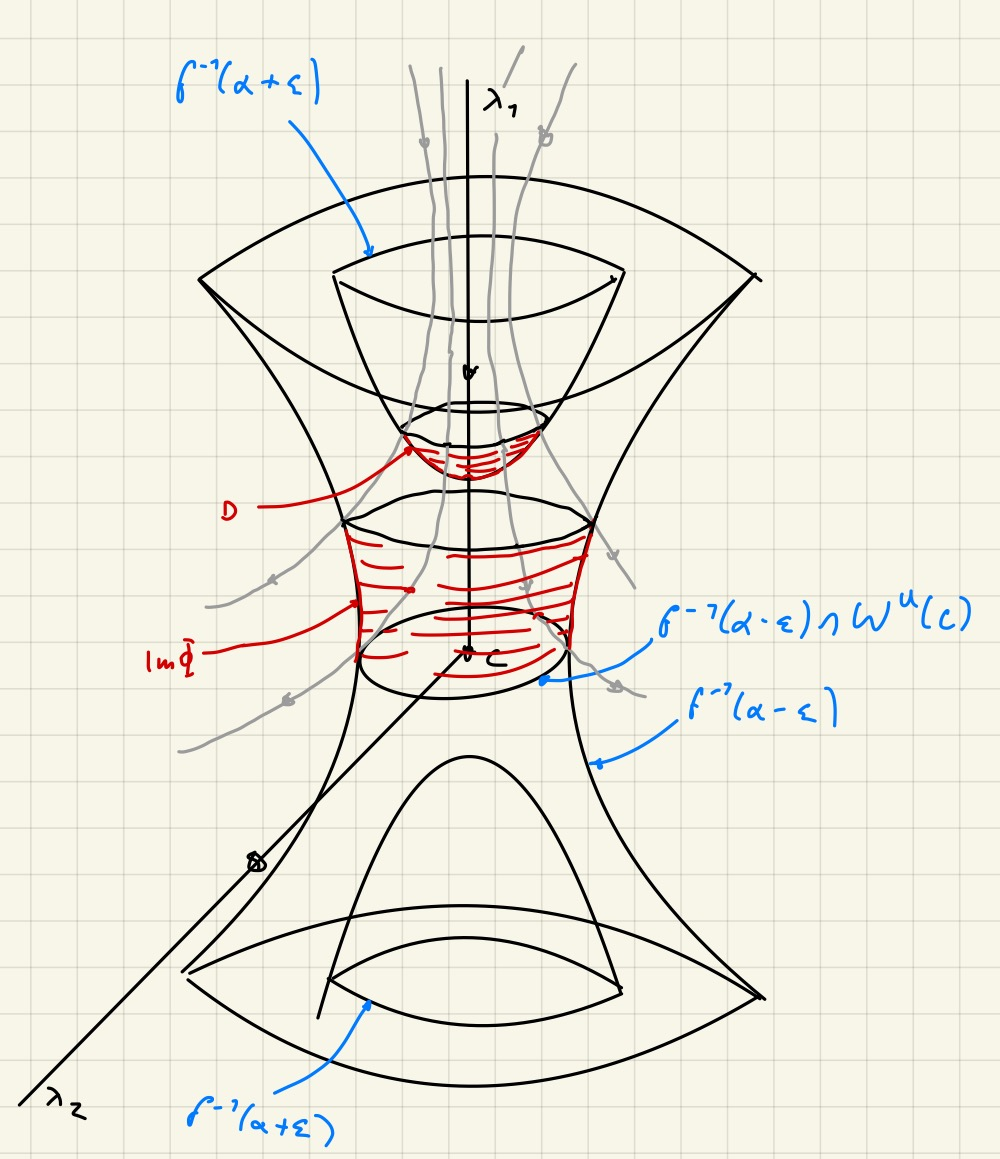
\includegraphics[width=.85\linewidth]{../resources/bew-gebrochene-trajektorien-sind-1-dim-mannigfaltigkeit-1.JPG}
          \captionof{figure}{A figure}
          \label{fig: test1}
        \end{minipage}%
        \begin{minipage}{.5\textwidth}
          \centering
          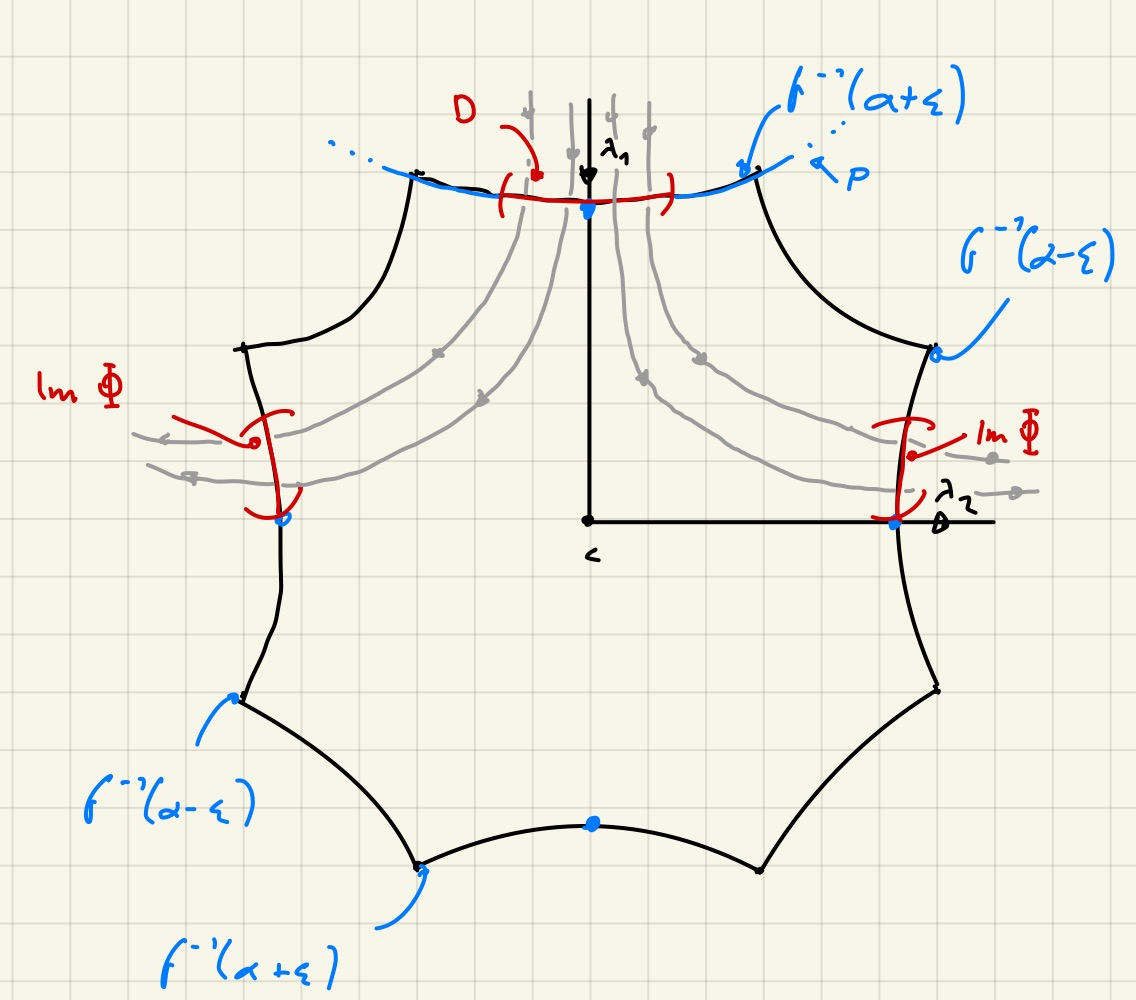
\includegraphics[width=.85\linewidth]{../resources/bew-gebrochene-trajektorien-sind-1-dim-mannigfaltigkeit-2.JPG}
          \captionof{figure}{Another figure}
          \label{fig: test2}
        \end{minipage}
    \end{figure}

    Man betrachte die Abbildungen~\ref{fig: test1} und~\ref{fig: test2}.

    $D$ ist eine Umgebung von dem Punkt $a_1$, an dem $\lambda_1$ auf den Rand der Morse Umgebung 
    trifft. Die Idee des Beweises ist es, die Menge $D - a_1$ entlang der Trajektorien von $X$ auf den 
    Teil des Randes der Morse Umgebung, an denen die Trajektorien austreten, via einer Abbildung $\Phi$ 
    zu projizieren. Fügen wir nun den Punkt $a_2$, an dem $\lambda_2$ auf den Rand der Morse Umgebung 
    trifft zum Bild dieser Menge hinzu, dann bekommen wir eine 1-dimensionale Mannigfaltigkeit mit Rand, 
    und der Rand ist $a_2$. Wir können also eine Umgebung von $a_2$ in $\Ima \Phi \cup a_2$ via einer
    Abbildung $\chi \colon [0, \delta)$ parametrisieren, aber in dieser Umgebung können wir auch jeden 
    Punkt mit einer Trajektorie in $\Lb (p, q)$ identifizieren.
\end{proof}
